\section{Einrichtung des ADS-Workspaces}

    \subsection{Auswahl der Technologie und Erstellung des Substrat-Files}
    Bevor wir in ADS die Leitungen Simulieren können, muss das Substrat file definiert werden.
    Hier lässt sich die dicke der Kupferleitung sowie von dem Dielektrikum FR4 wählen.
        \begin{itemize}
            \item FR4    : 1mm
            \item Kupfer : 35\textmu m
        \end{itemize}
        \begin{figure}[H]
            \centering
            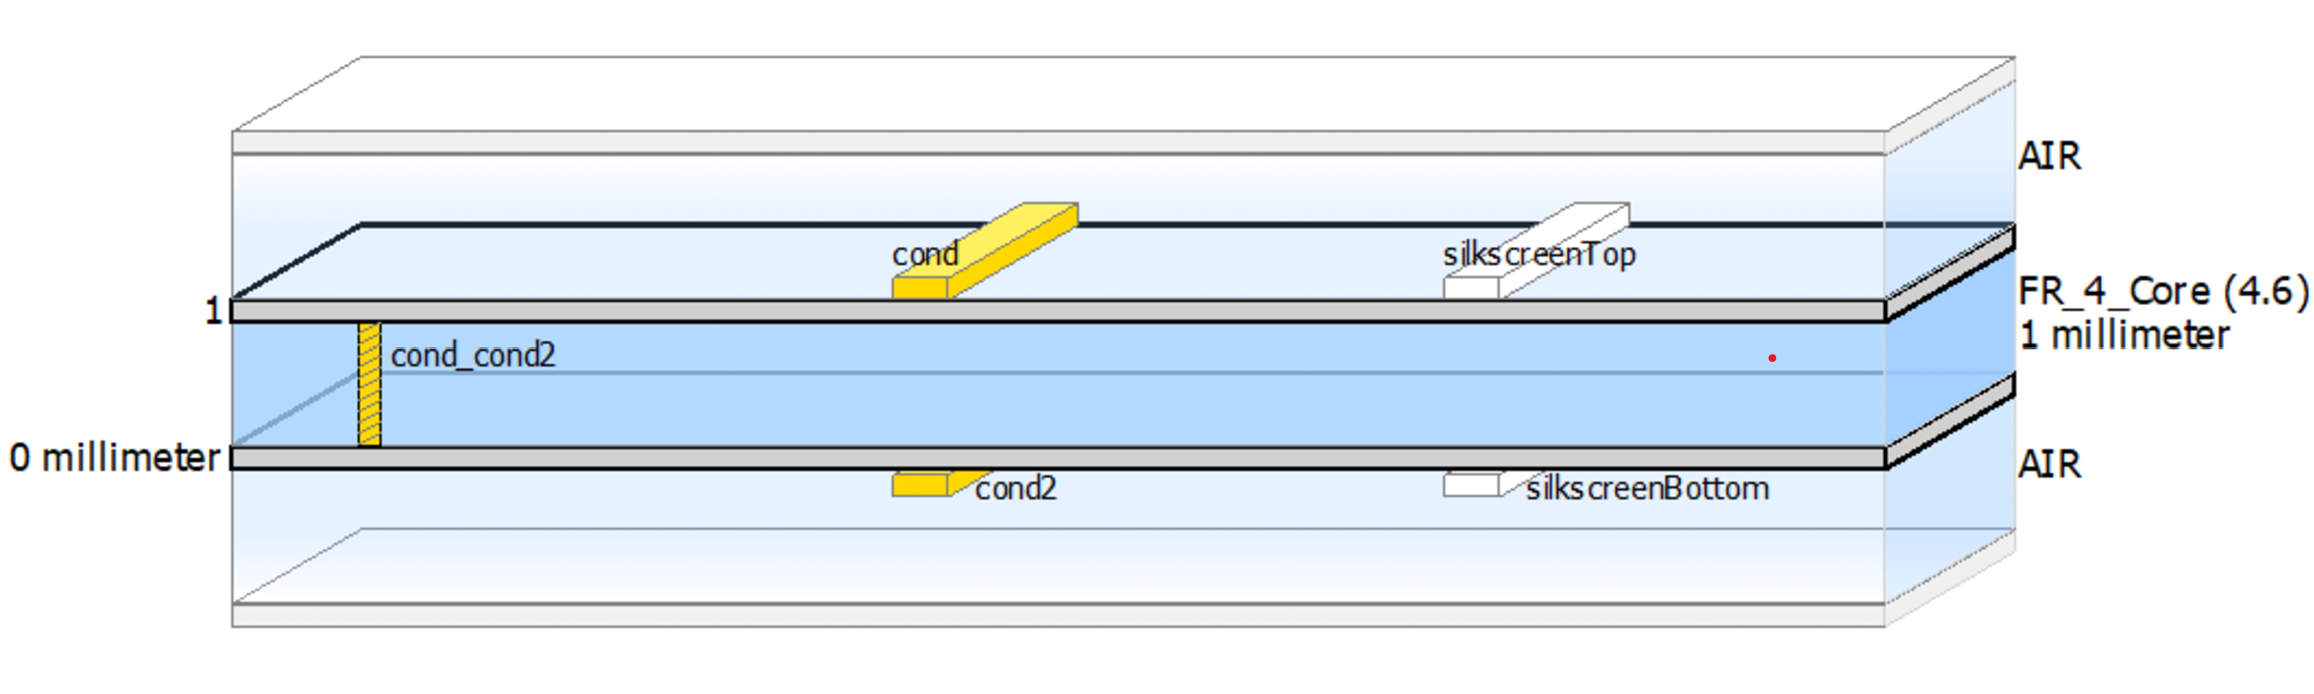
\includegraphics[width=0.9\textwidth]{Pictures/substratFile.png}
            \caption{Substratfile}
        \end{figure}

    \subsection{Nutzung des Controlled Impedance Line Designers}

\section{Leitungsdimensionierung}
    \subsection{\texorpdfstring{Berechnung der Leitungsbreite ($Z_0 = 50~\Omega$)}{Berechnung der Leitungsbreite (Z0 = 50 Ohm)}}
    Nun wird die Leitungsbreite einer Microstrip Leitung mit der Wellenimpedanz $Z_0 = 50~\Omega$ berechnet.
    Dazu verwenden wir die Formeln, die uns auf der Website von Microwaves101 Kapitel Microstrip zur
    Verfügung gestellt werden. Durch eine grobe Abmessung der Leitungsbreite sieht man das folgende Beziehung gilt: \\
    \[
    \frac{w}{h} \geq 1
    \]
    $w$ ist hier die Leitungsbreite und $h$ die Höhe des Dielektrikums. In unserem Fall ist $h = 1mm$ und $w$ wird variiert. Die 
    effektive Permitivität wird mit folgender Formel berechnet:
      \[
    \varepsilon_e = \frac{\varepsilon_r + 1}{2} + \frac{\varepsilon_r - 1}{2} \left( 1 + 12 \frac{h}{w} \right)^{-\frac{1}{2}}
    \]
   \\ $\varepsilon_e$ wird in die Formel zur Leitungsimpedanz eingesetzt. Bei dieser wird $w$
    variiert, bis die Wellenimpedanz $Z_0 = 50~\Omega$ erreicht wird.
    \\
    Die Formel zur Leistungsimpedanz $Z_o$ lautet:
    \[
    Z_0 = \frac{120 \pi}{\sqrt{\varepsilon_{\text{eff}}} \left( \frac{w}{h} + 1.393 + \frac{2}{3} \ln\left( \frac{w}{h} + 1.444 \right) \right)} \quad \text{(Ohm)}
    \]
    Die Berechnung der Leitungsbreite wird hierbei numerisch durchgeführt, da eine analytische Berechnung zu
    komplex werden würde. Die Ergebnisse der Approximation werden in Tablle 4.1 dargestellt. \\
    
    \begin{table}[H]
        \centering
        \begin{tabular}{|l|l|}
            \hline
            \textbf{Leitungsbreite $w$ (mm)} & \textbf{Wellenimpedanz $Z_0$ ($\Omega$)} \\
            \hline
            1.7 & 52.749 \\
            1.8 & 51.027 \\
            1.9 & 49.419 \\
            2.0 & 47.915 \\
           
            \hline
        \end{tabular}
        \caption{Berechnete Wellenimpedanz für verschiedene Leitungsbreiten}
    \end{table}
    Anhand der berechneten Werte liegt die Leitungsbreite mit $w = 1.8~mm$ am nähesten an der Wellenimpedanz.
    Eine nähere Berechnung ist mit unserem TR nicht möglich. 

       

    \subsection{Verifizierung der Berechneten Leitungsbreite}
    Nun wird die Leitungsbreite mithilfe des Controlled Impedance Line Designers Simuliert.
    Ziel ist es die $Z_0 = 50~\Omega$ zu erreichen durch sweepen der Leitungsbreite
    \begin{figure}[H]
        \centering
        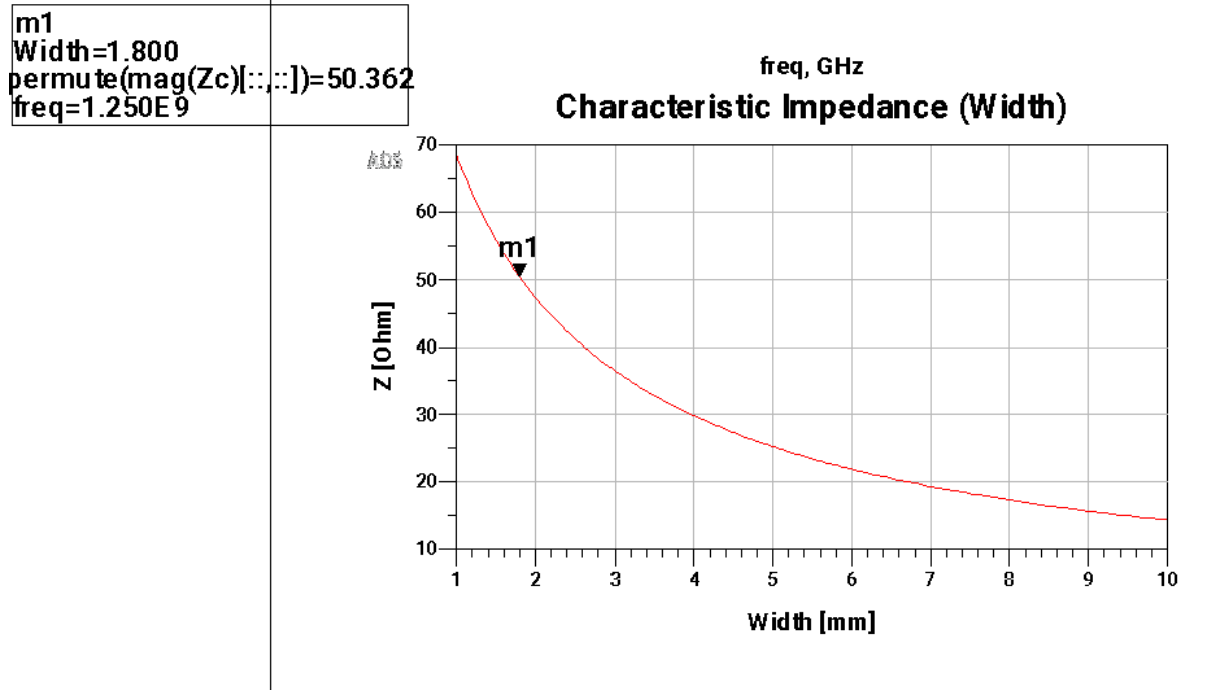
\includegraphics[width=0.8\textwidth]{Pictures/LeitungsbreitenSweep.png}
        \caption{Wellenimpedanz in abhängigkeit von der Leitungsbreite}
    \end{figure}
    Wie schon numerisch bestimmt kommen wir mitn der Leiterbreite $w=1.8mm$ der Wellenimpdanz $Z_0 = 50~\Omega$
    am nähesten. Würde man noch genauer sweepen, wird man festellen dass die Optimale Leiterbreite irgendwo zwischen
    $1.8mm$ und $1.9mm$ liegt.

    \subsection{Charakteristische Länge der Koppelleitungen}
    Die Gleichung für die Länge der Leitung wurde schon in \eqref{eq:laenge} hergeleitet.
    Gegebene Werte:
    \begin{align}
        \mu_r &= 1 \\
        c_0 &= 3 \cdot 10^8 \frac{m}{s}
    \end{align}

    Die Permitivität von Kufper kann nicht allgemein angegeben werden, sondern muss bestimmt werden. 
    Wir konnten mithilfe des "Controlled Impedance Line Designers" die Permitivität auf $\epsilon_r = 3.42631$ bestimmen 
    Damit lässt sich die Theoretische Leitung berrechnen.
    \begin{equation}
        L= \frac{c_0}{4 \cdot f_c \cdot \sqrt{\epsilon_r}} = 0.03241m = 32.41mm
        \label{eq:laenge}
    \end{equation}
    \clearpage
    Mithilfe von ADS konnten wir die Filtercharakteristik in abhängigkeit der Leitungslänge Simulieren. Durch das Sweepen der 
    Leitungslänge konnten wir folgendes Diagramm erstellen.
    \begin{figure}[H]
        \includegraphics[width=0.7\textwidth]{Pictures/SimulationSweepLängeS21.png}
        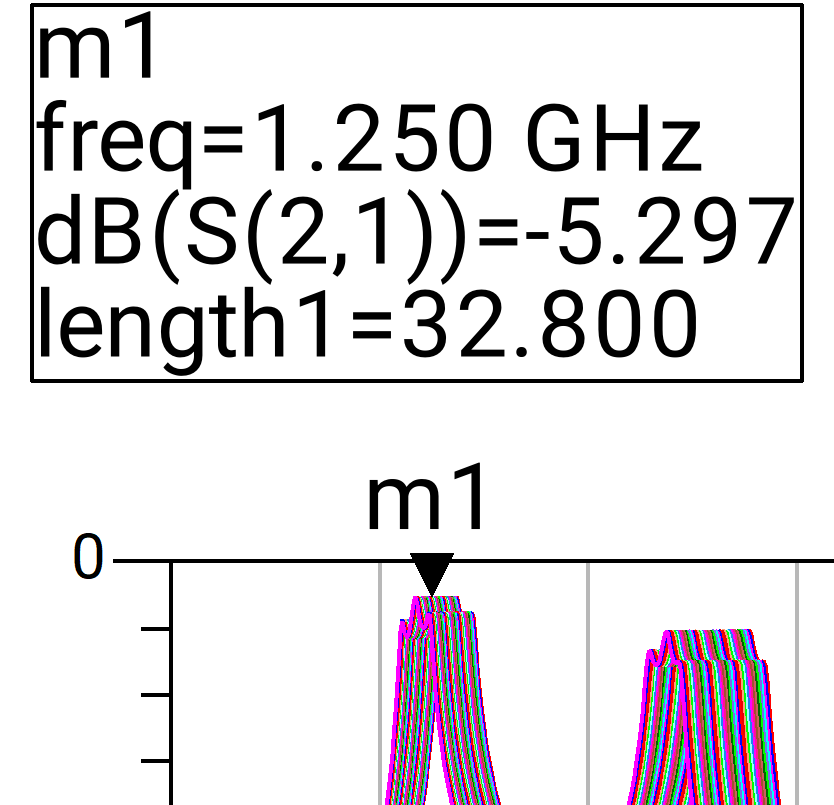
\includegraphics[width=0.3\textwidth]{Pictures/gezoomt.png}
        \centering
        \caption{Leitungslängensweep}
    \end{figure}
    Schauen wir uns den Filter bei 1.25Ghz an, dort sehen wir das wir die beste Filtercharteristik bei einer
    Leitungslänge von etwa $L=32.80mm$ haben.
    Was eine abweichung von etwa $0.4mm$ entspricht, das liegt mitunter an anderen 
    Simulationsmodellen und auch an der berücksichtigung von den vier Bandpassfiltern.

    \clearpage
    \section{Simulation im Vergleich zur Praxis}
    \begin{figure}[H]
        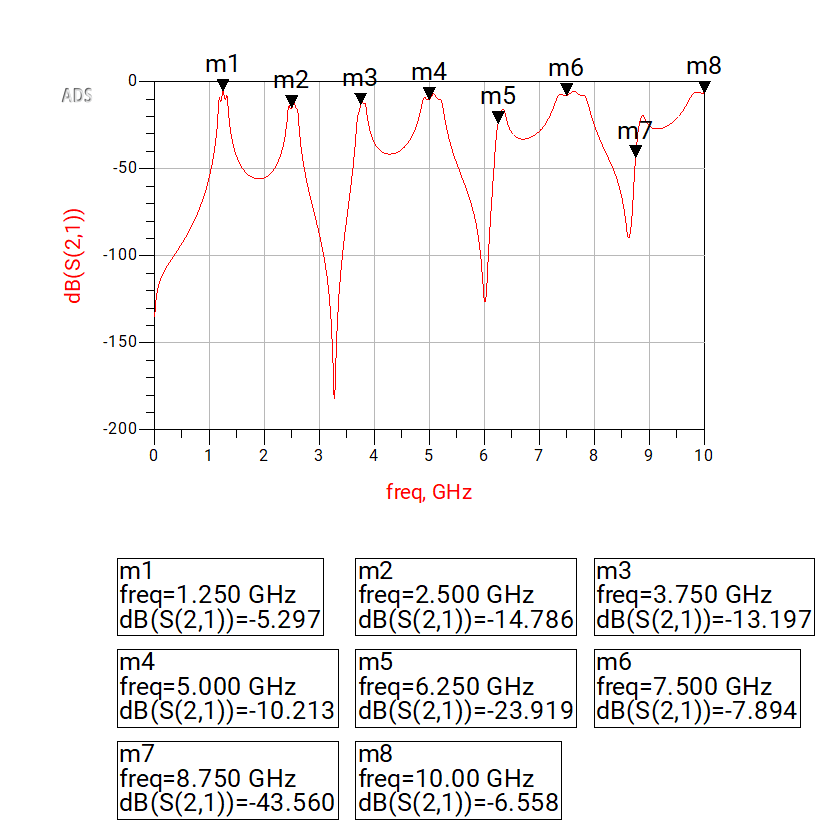
\includegraphics[width=0.7\textwidth]{Pictures/simulationmitmarkern32.8.png}
        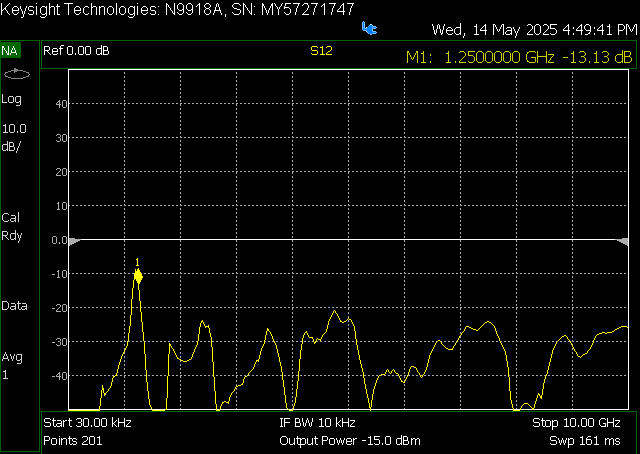
\includegraphics[width=0.7\textwidth]{Pictures/S12neuCooleGrupp.png}
        \centering
        \caption{Filtercharakteristik Praxis vs Simulation}
    \end{figure}
    In der Praxis lassen sich ebenso wie in der Theorie die Peaks,die ein Vielfachse von 1.25GHz sind sehen.
    Wenn wir uns in der Praxis die 1.25Ghz genauer anschauen, sehen wir das der Filter eine Dämpfung von -13.31dB
    aufweist in der Theorie jedoch nur -5.23dB. Dieser Fehler kommt duch die Dämpfung des Koaxialkabels
    das in der Theorie nicht berücksichtigt wurde.
    Nach Versuch 1 ist bekannt, dass die Dämpfung des Koaxialkabels bei 1.25GHz bei etwa -7.13dB liegt.
    Wird diese Dämpung vom Theorie wert abgezogen $D=-5.23dB-7.13dB=-12.36dB$, kommen wir dem Praktischen wert schon deutlich näher.




\section{Aufbau des Coupled-Line-Filters im Schematic}

\section{Simulation und Optimierung}
    \subsection{Vergleich mit Messdaten}

\section{Knick zur Optimierung des Aspektverhältnisses}

\section{Anpassung im Schematic und Re-Simulation}

\section{Auswirkungen auf die S-Parameter}
